%% Paper II of the split of docs/paper1 (docs/split_paper_tasks.md): data assimilation.
%% Target: JAMES (S0.2), AGU class.
\PassOptionsToPackage{natbibapa}{apacite}% keep \citet / \citep with apacite
\documentclass[draft]{PJ2019}

\usepackage{amsmath,amssymb}
\usepackage{amsthm}
\usepackage{mathtools}
\usepackage{bm}
\usepackage{booktabs}
\usepackage{xcolor}
\usepackage{xspace}
\usepackage[group-separator={,}]{siunitx}
\usepackage[hidelinks]{hyperref}

% Shared notation; copied from docs/paper1/macros.tex at the split (S1.5).
\newcommand{\DKY}{D_{\mathrm{KY}}}
\newcommand{\dlat}{d_{\mathrm{lat}}}
\newcommand{\Nens}{N_{\mathrm{ens}}}
\newcommand{\R}{\mathbb{R}}
\newcommand{\Z}{\mathbb{Z}}
\newcommand{\E}{\mathcal{E}}          % encoder
\newcommand{\Dec}{\mathcal{D}}        % decoder
\newcommand{\Fp}{\mathcal{F}}         % latent propagator
\newcommand{\Hobs}{\mathcal{H}}       % physical observation operator
\newcommand{\Lat}{\Lambda}            % site lattice
\newcommand{\Shift}{\mathsf{S}}       % lattice shift
\newcommand{\Tr}{\mathsf{T}}          % physical translation
\newcommand{\Exp}{\mathbb{E}}
\newcommand{\Var}{\operatorname{Var}}
\newcommand{\Cov}{\operatorname{Cov}}
\newcommand{\tr}{\operatorname{tr}}
\newcommand{\dist}{\operatorname{dist}}
\newcommand{\Renc}{R_{\mathrm{enc}}}
\newcommand{\Rdec}{R_{\mathrm{dec}}}
\newcommand{\Rprop}{R_{\mathrm{prop}}}
\newcommand{\kmax}{k_{\max}}
\newcommand{\kmid}{k_{\mathrm{mid}}}
\newcommand{\wvar}{w_{\mathrm{var}}}
\newcommand{\wld}{w_{\mathrm{ld}}}
\newcommand{\ie}{i.e.\@\xspace}
\newcommand{\eg}{e.g.\@\xspace}

\newtheorem{proposition}{Proposition}
\newtheorem{lemma}{Lemma}
\newtheorem{corollary}{Corollary}
\theoremstyle{remark}
\newtheorem{remark}{Remark}

% Run-in paragraph heading (revtex letters \paragraph headings; we do not want that).
\newcommand{\para}[1]{\par\medskip\noindent\textbf{#1}\enspace}

% Wide table: full line width with the columns spread out (like revtex's ruledtabular) when it fits,
% shrunk to the line width only when its natural width is larger -- never enlarged, so a narrow table
% keeps the float font size (fixed 2026-10-11: \resizebox alone scaled small tables up).
% #1: column spec, #2: body (header + rows). The body is typeset twice (measured, then set).
\makeatletter
\newsavebox\wt@box
\newcommand{\widetabular}[2]{%
  \sbox\wt@box{\begin{tabular}{#1}\hline\hline\noalign{\vskip 2pt}#2\noalign{\vskip 2pt}\hline\hline\end{tabular}}%
  \ifdim\wd\wt@box>\linewidth
    \resizebox{\linewidth}{!}{\usebox\wt@box}%
  \else
    \begin{tabular*}{\linewidth}{@{\extracolsep{\fill}}#1}\hline\hline\noalign{\vskip 2pt}#2\noalign{\vskip 2pt}\hline\hline\end{tabular*}%
  \fi}
\makeatother
% Table bodies are read with TeX's primitive \input (expandable), so a rule may follow them.
\makeatletter\newcommand{\tabinput}[1]{\@@input #1.tex }\makeatother

% REVTeX's ruledtabular (used by every table) for non-REVTeX classes: centred table with
% double rules above and below; the table body supplies its own \hline after the header.
\makeatletter
\@ifundefined{ruledtabular}{%
\newenvironment{ruledtabular}{\par\centering
  \let\rt@tabular\tabular \let\rt@endtabular\endtabular
  \renewenvironment{tabular}[1]{\rt@tabular{##1}\hline\hline\noalign{\vskip2pt}}%
    {\noalign{\vskip2pt}\hline\hline\rt@endtabular}}{\par}}{}
\makeatother

% Placeholder for numbers that pending runs will fill (Block K; see docs/paper1/partII_narrative.md,
% table P1-P12). Renders in red so none survives into a submitted draft unnoticed.
\providecommand{\textcolor}[2]{#2}
\newcommand{\placeholder}[1]{\textcolor{red}{\textbf{[#1]}}}


% Float placement for a single-column draft: let figures and tables sit near their first
% mention (the REVTeX top-only placement pushed most of them to the end of the paper).
\renewcommand{\topfraction}{0.9}
\renewcommand{\bottomfraction}{0.8}
\renewcommand{\textfraction}{0.07}
\renewcommand{\floatpagefraction}{0.75}
\setcounter{topnumber}{3}
\setcounter{bottomnumber}{2}
\setcounter{totalnumber}{5}

\journalname{Journal of Advances in Modeling Earth Systems (JAMES)}

\begin{document}

\title{Exactly local ensemble data assimilation in a learned latent field}

\authors{Dalton Jones\affil{1}, Peter Jan van Leeuwen\affil{1}}

\affiliation{1}{Department of Atmospheric Science, Colorado State University, Fort Collins, USA}

\correspondingauthor{Dalton Jones}{daltjone@colostate.edu}

% Key points: AGU limit of three, at most 140 characters each, no special characters.
\begin{keypoints}
\item A filter in a learned local latent field is exactly local; four shifted lattices cut its error by 30 percent; its nonlinearity costs little
\item One learned model trained only on noisy data and one filter setting give the same analysis error on domains from 44 by 44 to 440 by 440
\item The learned filter beat physics filters with parameter estimation only for errors of model form, not for wrong parameters
\end{keypoints}

\begin{abstract}
Latent-space ensemble data assimilation has so far used a global latent vector, which has no
notion of distance, so the filter cannot be localized and its ensemble grows with the domain's
unstable directions. We instead assimilate in a
learned latent field, a few channels per site of a lattice tiling the domain, whose
weight-shared local operators run on domains of any size (companion
paper). With a decoder that reconstructs each patch from its own site, the latent observation
operator is exactly local, and a per-site latent ensemble Kalman filter uses it untruncated.
Blending analyses on four copies of the patch lattice shifted by half a patch lowers the error by about $30\%$.
The decoder's nonlinearity costs little (the term the filter neglects is $4\%$ of the observation
error); keeping members in the decoder's range costs more.
In twin experiments with the
two-dimensional Kuramoto--Sivashinsky equation, one model trained only on noisy fields and one
filter setting give errors of $0.30$--$0.33$ on every domain from $44^2$ to $440^2$,
against $0.82$ for interpolation; an unlocalized filter fails once unstable directions outnumber members.
Against physics-based filters with wrong models, given online parameter estimation and bias
correction, the latent filter loses or ties when the error is in a parameter or a bias, and, in the
configuration tested, wins when it is in the form of the equations and exceeds about a quarter to a third of
the observation error after the remedy.
In Kolmogorov flow its errors are $43\%$ below interpolation.
\end{abstract}

\section*{Plain Language Summary}
Weather forecasts start from an estimate of the atmosphere's current state that combines a
forecast model with observations: data assimilation. The most widely used methods run
a small set of forecasts and treat each region separately, so few forecasts suffice however
large the domain. Machine-learned forecast models usually describe the
whole state by one list of numbers with no notion of where things are, so they cannot be
treated region by region. We use a learned model that keeps a map: a few numbers
at each point of a coarse grid, updated by the same local rule everywhere. Each grid point then
depends only on nearby observations, the method works the same way on domains a hundred times
apart in size, and the model can be trained on noisy data alone. The model's nonlinear
link to the physical field could mislead the method; we found the effect small. When the
physical model used for comparison had an equation of the wrong form, the learned model did better
in our tests once that error exceeded about a quarter to a third of the measurement error; when only
a parameter was wrong, or the model was accurate, the physical model remained better.

%======================================================================
\section{Introduction}
\label{sec:introduction}
%======================================================================

Ensemble filters estimate the uncertainty of a forecast from a small
ensemble of model runs, and in high-dimensional systems they work only
because of localization: each region is analysed from nearby observations
with covariances estimated from the ensemble, and distant, spurious
correlations are suppressed \citep{houtekamermitchell2001,ott2004,hunt2007}.
The case for it is strongest in spatially extended chaos. There the forecast
errors within a region span few directions \citep{patil2001}, while the
number of unstable directions of the whole attractor, like its
Kaplan--Yorke dimension $\DKY$, grows in proportion to the domain
\citep{ruelle1982,manneville1985,egolfgreenside1994}. A filter without
localization needs at least as many members as there are unstable and
neutral directions \citep{bocquetcarrassi2017,takeda2026}, so its ensemble
must grow with the domain; a localized one needs only enough members for
the directions inside its local region.

Data assimilation in a learned latent space has so far given up this
remedy. Filters in the latent space of an autoencoder compress the whole
field into one latent vector and estimate its covariance from the ensemble
\citep{peyron2021,chen2023roadenkf,pasmans2025,tong2026laeenkf,si2025latentensf}.
A latent vector has no notion of distance, so there is nothing to taper:
recent latent filters either do not localize or leave localization for
future work \citep{chen2023roadenkf,tong2026laeenkf}, and the dimension of
the vector, fixed at training time, ties the model to one domain size. For
the large, extensively chaotic domains on which ensemble data
assimilation is used in practice, both are limits of principle rather than
of implementation.

A companion paper \citep[hereafter Paper~I]{jones2026transfer} makes the latent a
\emph{field}: a few channels at each site of a lattice that tiles the
domain, encoded, decoded and propagated by operators that are shared by
all sites and read a bounded neighbourhood. One trained model therefore
runs on a domain of any size by adding sites. Paper~I validates this
transfer against the model's own Lyapunov spectrum: trained on a small periodic
box or on windows of one large simulation, Paper~I's two-dimensional Kuramoto--Sivashinsky (KS)
models reproduce the true $\DKY$ to within $3.5\%$ at $44^2$ and $66^2$ (this paper's noisy-trained model:
$+3.6\%$ and $-2.1\%$, Table~\ref{tab:model_validation}), and
Kolmogorov flow needs the window route. A latent field has a geometry, and this paper asks
what that geometry is worth to an ensemble filter.

The answer has three parts. First, locality can be made exact: with a
decoder that reconstructs each patch from its own site, the observations
of a patch depend on that site alone, the latent observation operator is
block-diagonal, and a per-site ensemble filter in the latent space
needs no truncation of it. Second, the error that exact locality
leaves, tied to the patch lattice, is removed by running the filter on
shifted copies of the lattice and blending the analyses, without
retraining. Third, the localized filter keeps its accuracy and its
ensemble size as the domain grows, because both are set by the local
problem. These are properties of the method. Whether to use a learned
model at all is a separate question, because a filter built on the
correct equations is far more accurate than one built on a learned
surrogate. Models of real systems are not correct, however, and for many
systems, convection-permitting models of the atmosphere among them, the
errors are structural and poorly known, while the errors of the
observations are well characterized. We therefore train the model only on
noisy fields and compare it with physics-based filters whose models are
wrong in controlled ways and which are given the standard remedies for
model error.

\para{Contributions.}
\begin{itemize}
\item \emph{Exact locality in a learned latent space}
  (Sec.~\ref{sec:method}). With a per-patch decoder the latent observation
  Jacobian is block-diagonal (Proposition~\ref{prop:blockdiag}) and is
  obtained from as many forward passes as there are channels, at any
  domain size.
\item \emph{Shifted tilings} (Sec.~\ref{sec:da_tilings}). Four copies of the
  patch lattice shifted by half a patch, blended with smooth weights, lower
  the analysis error by about $30\%$ with the same model; the gain comes
  from the offsets, not from the extra members.
\item \emph{One model and one setting from $44^2$ to $440^2$}
  (Sec.~\ref{sec:da_2d}). In 2D KS the analysis error is $0.30$--$0.33$ on
  every domain over a factor of 100 in area, against $0.81$--$0.83$ for
  interpolating the observations, with an ensemble that saturates at
  about 32 members per tiling at both sizes tested, while an unlocalized filter
  fails once the attractor has more unstable directions than the ensemble
  has members.
\item \emph{What the nonlinear decoder costs} (Sec.~\ref{sec:da_nonlinear}).
  Observed through the decoder, the latent observation operator is
  nonlinear even for linear observations, and the filter linearizes it. At
  the native configuration the neglected term is about $4\%$ of the
  observation error, and relinearizing the update changes the error by at
  most $0.001$. With the true equations as forecast and the members in the
  decoder's range, the filter is no better than with the learned model; the
  error comes from the decoder's range, which costs about half of it, not
  from the learned dynamics or the nonlinearity.
\item \emph{Learned versus physics-based filters}
  (Sec.~\ref{sec:da_model_error}). The latent filter loses to a
  physics-based filter whose model error lies in a parameter or a bias,
  at every magnitude tested, once online parameter estimation is working, and wins when
  the error lies in the form of the equations and the part bias correction
  cannot remove exceeds about a quarter to a third of the observation error after the remedy,
  in the configuration tested. A missing process of
  increasing strength, tuned for on both sides, gives a tie just below that
  point and wins of $1.27$ and $1.29$ times above it.
\item \emph{Training on noisy data} (Sec.~\ref{sec:da_noisy}). The model is
  trained only on complete fields that carry observation-level noise, and
  assimilates at least as well as the same model trained on clean fields
  ($4$--$5\%$ lower error at every size, below the $10\%$ of our decision rule).
\end{itemize}

All experiments are twin experiments. The main system is 2D KS
(Sec.~\ref{sec:system}); 1D KS shows how the ensemble an unlocalized filter
needs grows with the domain and that a distance taper beats a distance-free
correction (Sec.~\ref{sec:da_1d}), and Kolmogorov flow shows that the
filter carries over to chaos organized by a forcing
(Sec.~\ref{sec:kolmogorov_da}). The target we have in mind is the
assimilation of convection-permitting simulations of organized convection,
where the equations of the cloud processes are uncertain and the domain is
set by the application. Section~\ref{sec:background} reviews the
background, Sec.~\ref{sec:method} the model and the filter, and
Secs.~\ref{sec:da_results}--\ref{sec:kolmogorov_da} the results;
Sec.~\ref{sec:discussion} discusses them and their limitations.

%======================================================================
\section{Background}
%======================================================================
% TODO(S4.3): paper1 §2.3, expanded; new prior-work table.
\placeholder{S4.3: Background}

%======================================================================
\section{Method}
%======================================================================
% TODO(S4.4--S4.5): §3.1 restated latent field; §3.2--3.5 paper1 §3.8 (Prop. 4 -> Prop. 1).
\placeholder{S4.4--S4.5: Method}

%======================================================================
\section{System, model and ground truth}
\label{sec:system}
%======================================================================

%----------------------------------------------------------------------
\subsection{Two-dimensional Kuramoto--Sivashinsky}
\label{sec:ks2d}
%----------------------------------------------------------------------

The 2D experiments use the isotropic Kuramoto--Sivashinsky (KS) equation
\citep{kuramoto1976,sivashinsky1977,kalogirou2015},
\begin{equation}
  u_t + \nabla^2 u + \nabla^4 u + \tfrac12|\nabla u|^2 = 0,
  \qquad (x,y)\in[0,L)^2,
  \label{eq:ks2d}
\end{equation}
whose linear growth rate $K^2-K^4$ is positive on the ring $|\bm k|<1$ and
largest at $|\bm k|=1/\sqrt2$, which sets a pattern wavelength of
$2\sqrt2\,\pi\approx8.9$. Its nonlinearity drives the spatial mean of
$u$, which carries no dynamical information (only gradients of $u$ enter
the right-hand side), so we project the $\bm k=0$ mode out after every
step. The equation is integrated in Fourier space with a fourth-order
exponential time-differencing Runge--Kutta scheme (ETDRK4,
\citealp{kassam2005}) in double precision, with solver step $0.02$,
snapshot interval $\Delta t=0.1$ and grid spacing $\Delta x=0.344$
($128$ points at $L=44$). Figure~\ref{fig:systems} shows the domain whose
windows train the model.

The training data are four trajectories (plus one for validation) of 25
time units on a single periodic domain of side $264=6\times44$ ($768^2$
points), after a spin-up of 200 time units. The model is deployed on
square periodic domains of side $44$, $66$, $88$, $220$, $330$ and $440$, which
are all multiples of the site length $h=5.5$.

\para{Ground truth.} The Lyapunov spectrum of the PDE is computed with
the Benettin algorithm \citep{benettin1980} and the exact tangent
dynamics of the time-stepper, over 40-unit windows (about 7 Lyapunov
times) after a spin-up of 200 time units (protocol in
Appendix~\ref{app:groundtruth} and Paper~I). At $44^2$ three independent
runs give $\DKY=80.7$, $81.8$ and $83.6$ (mean $82.0$), with $42$--$44$ positive
exponents and $\lambda_1=0.165$--$0.194$; at $66^2$ two runs give $185.6$ and
$192.5$ (mean $189.0$), with $93$--$101$ positive exponents. The densities,
$0.0424$ and $0.0434$ per unit area, differ by $2.5\%$, inside the spread of
the individual runs, and the running estimates still move by $3$--$5\%$ over
the last 20 time units, so we treat the truths as uncertain at the level
of a few percent. Larger domains are beyond a full Lyapunov computation
(the expected dimension at $88^2$ is about 330); there the evidence that the
model remains faithful is the filter's own behaviour
(Sec.~\ref{sec:da_2d}) and the transfer results of Paper~I.

\begin{figure}[htbp]
\centering
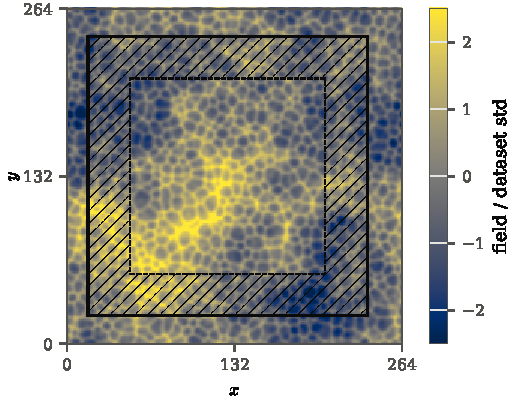
\includegraphics{figures/systems_ks2d.pdf}
\caption{One snapshot of 2D KS on the $264^2$ periodic domain whose
windows train the model, divided by the training standard deviation. The
outlined square is one $40\times40$-site training window, its forced halo
(six sites) hatched and its free interior inside the dashed line. Cells of
a fixed size fill the domain, which therefore holds many independent
copies of the local dynamics; this is what window training samples. The
training fields of the model used here additionally carry noise of
standard deviation $0.1$ (not shown).}
\label{fig:systems}
\end{figure}

%----------------------------------------------------------------------
\subsection{The model and its validation}
\label{sec:model_validation}
%----------------------------------------------------------------------

All 2D experiments use one model: the architecture and window training of
Paper~I with $c=12$ channels per site instead of 6, patches of $16\times16$
grid points ($h=5.5$), a propagator reach of $6$ sites, and the noisy
training of Sec.~\ref{sec:local_field} (settings in
Table~\ref{tab:architecture}). On a $44^2$ domain it has $64$ sites and
$\dlat=768$ latent coordinates; on $440^2$, $6400$ sites and $76\,800$, with the
same weights. We use 12 channels rather than the 6 of Paper~I because the
filter benefits from the extra capacity.

Table~\ref{tab:model_validation} compares the model with the truth.
Its Kaplan--Yorke dimension is $84.7$ at $44^2$ and $188.5$ at $66^2$, $3.6\%$ above
and $2.1\%$ below the truth run from the same initial condition; at $44^2$ it
lies just above the range of the three truth runs, at $66^2$ inside the
range of the two. Its number of positive exponents, $43$ and $94$, is inside
the truth's range at both sizes. Its leading exponent, $0.221$ and $0.217$, is
larger than the truth's ($0.165$--$0.194$ and $0.189$--$0.204$): errors grow
somewhat faster in the model than in the PDE. In free rollouts of 1000 steps
its field standard deviation is $5$--$7\%$ above the truth's from the same
initial conditions, and it carries slightly too much energy at the
smallest scales. A clean-trained model with the same recipe is as close to
the truth; Sec.~\ref{sec:da_noisy} compares the two as filters. Scored the
same way, the 6-channel model of Paper~I is within $1.7\%$ and $2.4\%$ at the
same two sizes (Paper~I reports $2.0\%$ and $0.6\%$ as means over initial
conditions against the mean truths).

\begin{table*}[htbp]
\caption{Validation of the 12-channel 2D KS models against the PDE. The
model's Kaplan--Yorke dimension, leading exponent $\lambda_1$ and number of
positive exponents $n_+$ are from one initial condition (seed 0); the error is
relative to the truth run from the same initial condition, and the truth
columns give the range over the independent truth runs (three at $44^2$, two
at $66^2$). Free rollout: field standard deviation (field units) and the share
of energy at $|\bm k|\ge1.4$ (\%), model / truth, from two initial conditions,
steps 100--1000 of 1000. Noisy-trained: the model of every experiment in
this paper.}
\label{tab:model_validation}
\widetabular{llccccccccc}{
Model & Size & $\DKY$ & Error & Truth $\DKY$ & $\lambda_1$ & Truth $\lambda_1$ & $n_+$ & Truth $n_+$ & Std & Small-scale energy \\
\hline
\tabinput{tables/model_validation}}
\end{table*}

%----------------------------------------------------------------------
\subsection{One-dimensional Kuramoto--Sivashinsky}
\label{sec:ks1d}
%----------------------------------------------------------------------

Section~\ref{sec:da_1d} uses the 1D equation,
$u_t + u u_x + u_{xx} + u_{xxxx} = 0$ on $[0,L)$, and the 1D model of
Paper~I, trained on whole periodic domains of length $L=100$ (grid spacing
$0.39$, snapshot interval $\Delta t=1.0$), with $16$ sites of length $6.25$,
$c=3$ channels, and an encoder and decoder that mix six neighbouring sites
($\Renc=\Rdec=6$). Its decoder is therefore not per-patch, and
Proposition~\ref{prop:blockdiag} does not apply; the 1D filters localize
the latent covariance instead (Appendix~\ref{app:da_filters}). Paper~I shows
that this model transfers to $L=200$ and $400$ with its $\DKY$ within about one
percent of the truth's. The truth has $\DKY=45.2$ and $26$--$27$ positive exponents
at $L=200$, and $\DKY=89.6$ and $51$ positive exponents at $L=400$, so the number of
unstable directions doubles with the domain.

%======================================================================
\section{Shifted tilings and one model from $44^2$ to $440^2$}
%======================================================================
% TODO(S4.7--S4.9): paper1 §7.1--7.4.
\placeholder{S4.7--S4.9: Shifted tilings and one model from $44^2$ to $440^2$}

%======================================================================
\section{Learned versus physics-based filters under model error}
\label{sec:da_model_error}
%======================================================================

No forecast model of a real system is correct, and for many systems of
interest, convection-permitting weather models among them, the model
error is large, structural and poorly known. Measurement error, by
contrast, is usually well characterized, which is why the model of this
section is trained on noisy fields. The question is then not whether a
learned filter beats a filter that knows the equations; with the true
equations the physics-based filter reaches $0.076$, four times better than
the latent filter's $0.31$. It is how wrong a physical model has to be
before a model learned from noisy data is the better choice, once the
physics-based filter is given every standard remedy for model error.

\para{Design.} The truth is the 2D KS equation, the system the latent
model was trained on, and its error, $0.312$ averaged over seeds 0--2
($0.302$--$0.324$), is fixed: it was not tuned for this section. The
comparator is the physical-space local ensemble transform filter of
Sec.~\ref{sec:comparator}, with the same observations and 64 members, whose forecast
model is wrong in one of four ways (Appendix~\ref{app:da_comparator}):
\begin{itemize}
\item \emph{a wrong coefficient}, $a\nabla^2u$ with $a=1.1$ or $1.25$;
\item \emph{a spurious process}: uniform advection at speed $1$ or $2$, or a
  fixed terrain-like forcing of amplitude $0.2$ or $0.4$;
\item \emph{a coarse grid}, $64^2$ or $32^2$ instead of $128^2$;
\item \emph{a wrong form of the damping}: $-a\nabla^2u - b(-\nabla^2)^{\gamma/2}u -
  (g/2)|\nabla u|^2$ with damping order $\gamma=5$, $6$ or $8$ instead of $4$, whose three
  coefficients are all estimated online, so that no coefficient is left
  wrong but no setting of them reproduces the KS growth-rate curve.
\end{itemize}
Each physics-based filter is given, and tuned on seed 0 over, the RTPS
weight and the localization radius; online estimation of the parameter
it gets wrong (the coefficient, the advection speed, or $a$, $b$ and $g$
jointly); and bias correction with additive model error estimated
offline from one-cycle residuals on an independent trajectory. Its
reported value is its best configuration on seed 0, confirmed on seeds
1--2; the decision rule (a filter wins if its three-seed mean is at least
$10\%$ lower and it is lower on every seed) was written down before the
runs. One further pre-registered case was stopped before its latent runs: a
missing cubic saturation, truth $u_t=\mathrm{KS}(u)-\beta u'^3$ with $u'$ the
mean-removed field. At the pre-registered strength its one-cycle error was
$0.055$ ($0.050$ state-dependent), and the physics-based filter without
remedies reached $0.190$ on seed 0, a physics win in line with the crossover
below; at no strength we tried did the state-dependent part exceed $0.06$
(the truth stopped being chaotic first), so the process could not test the
other side, and the anisotropic missing process below replaced it.

\para{Results.} Table~\ref{tab:da_model_error} and Fig.~\ref{fig:model_error} order the cases by the
physics-based filter's difficulty. It wins clearly when its model error
is one it can correct: with the $\nabla^2$ coefficient $10\%$ off and estimated
online it reaches $0.225$; bias correction removes the fixed forcing
entirely ($0.225$ at both amplitudes); and the coarse grids lose little
($0.083$ and $0.181$; bias correction does not help there). It loses when the error is larger or of the wrong form:
with the coefficient $25\%$ off, online estimation brings it from $0.48$ to
$0.42$, still $1.35$ times the latent filter's error; with spurious
advection, estimation of the speed leaves $0.44$ and $0.55$, $1.4$ and $1.8$
times. With the wrong damping order, where no coefficient is left wrong, the tuned
filter reaches $0.283$, $0.343$ and $0.409$ for $\gamma = 5$, $6$ and $8$. Joint online
estimation of $a$, $b$ and $g$ brings orders 5 and 6 to $0.263$ and $0.322$ and
does not help order 8: the physics-based filter wins at $\gamma=5$ ($1.19$ times),
ties at $\gamma=6$, and loses at $\gamma=8$ ($1.31$ times); bias
correction does nothing for these state-dependent errors ($0.297$, $0.361$
and $0.440$ on seed 0).

\para{The crossover.} What decides the comparison is not the size of the
physics model's one-cycle forecast error but its \emph{state-dependent}
part: the residual left after subtracting the mean one-cycle error,
which bias correction removes. The fixed forcing of amplitude $0.4$ has a
one-cycle error of $0.20$, but only $0.016$ of it is state-dependent, and the
physics-based filter wins. Every case whose state-dependent one-cycle
error is below $0.08$ (the grids, the forcing, the $10\%$ coefficient, damping
order 5, $0.000$--$0.077$) is a win or a tie for the physics-based filter; every
case at about $0.2$ or above (the $25\%$ coefficient, the advection, damping order
8) is a win for the latent filter; and order 6, at $0.12$, is a tie. In
this configuration the crossover therefore lies between $0.08$ and $0.2$ in
field units, near $0.1$, about a sixth of the observation error: a physical
model whose one-cycle error after bias correction is above it lost to the
model learned from data, and one below it did not. This is a result for one
system, one observation network, one cycle length, one ensemble size and one
learned model, not a general constant. The latent filter's error, which sets
the other side of the comparison, depends on all of them: it is $0.226$ with
observations twice as dense and $0.769$ with half as dense
(Sec.~\ref{sec:da_robust}). Nor does the crossover compare forecast errors
alone. The learned model's own one-cycle error, from the encoded true state
and including its decoder floor, is $0.19$ (Sec.~\ref{sec:da_accuracy}), larger
than that of a physics model it ties with (damping order 6, $0.12$
state-dependent): the outcome also depends on how each filter handles its
model's error, through its inflation and its remedies, not only on the size
of that error.
A separate question is a truth that is not Markov in the observed field, which
neither filter's model can represent: an
unobserved field $v$ with its own slow dynamics, $u_t=\mathrm{KS}(u)+\varepsilon v$,
$v_t=-v/\tau+\kappa\nabla^2u$, $\tau=2$, whose memory (4--4.5 time units, eight to nine cycles) makes $v$ a
function of the past of $u$, not of its present: about $20\%$ of its variance is not predictable from
the current field. This case does not test the crossover. The latent propagator maps the current
latent state to the next, so it is Markov by construction and cannot represent the memory either;
it is trained on noisy fields $u$ of this coupled system but never sees $v$. And because $v$ is
driven by $\nabla^2u$, much of its effect on $u$ looks like a change in the $\nabla^2$ coefficient,
which the physics-based filter, given every remedy (Appendix~\ref{app:da_comparator}), can estimate
online (it settles at $1.09$--$1.20$). The physics model's
error is therefore largely parametric, while the latent model's is structural. At $\varepsilon=0.1$
the latent filter's error is $0.476$ ($0.465$--$0.483$) and the physics-based filter's best, with
the $\nabla^2$ coefficient estimated online, $0.442$ ($0.436$--$0.447$); at $\varepsilon=0.2$ they are
$0.628$ ($0.620$--$0.641$) and $0.599$ ($0.596$--$0.604$). Both are ties by the decision rule, and
both filters lose ground against what the true equations achieve with $v$ unobserved ($0.405$ and
$0.493$, the same filter carrying its own $v$); both stay well below interpolation. Memory of this
kind limits a Markov latent model as much as a misspecified physical one, and the remedy on the
learned side, a propagator given past states, is outside this study.
\para{A missing process.} The hidden field does not test the crossover; a missing process that is
Markov in $u$ does. The truth adds an anisotropic gradient nonlinearity,
$u_t=\mathrm{KS}(u)-\tfrac{\delta}{2}(u_x^2-u_y^2)$ with $\delta=0.1$, $0.2$ and $0.3$, and the
physics-based filter's model is the isotropic KS equation. Joint online estimation of $a$, $b$ and $g$
cannot represent a term that tells $x$ from $y$, so this error is structural, like the wrong damping
order, but its size is set by one parameter. The latent model is retrained on noisy fields of each truth
with the same recipe, and the latent filter keeps its single setting; the errors are in that system's field
units. The physics-based filter was tuned over the full grid of Appendix~\ref{app:da_comparator} on seed
0, with every remedy at its best setting, and so was a filter with the true equations, which reaches
$0.087$, $0.087$ and $0.096$. The state-dependent one-cycle errors are $0.094$, $0.194$ and $0.323$, that is
$0.15$, $0.31$ and $0.49$ of the observation error, so the three levels straddle the crossover found above.
The outcome is the one the crossover predicts (Table~\ref{tab:da_model_error}, squares in
Fig.~\ref{fig:model_error}a). At $\delta=0.1$ the latent filter's error is $0.310$ ($0.300$--$0.323$) and
the physics-based filter's $0.328$ ($0.324$--$0.333$): lower on every seed, but by $5.5\%$, a tie. At
$\delta=0.2$ they are $0.341$ ($0.337$--$0.345$) and $0.433$ ($0.427$--$0.440$), and at $\delta=0.3$
$0.376$ ($0.372$--$0.383$) and $0.485$ ($0.470$--$0.496$): the latent filter wins by $1.27$ and $1.29$
times. Online estimation of $a$, $b$ and $g$ lowered the physics-based filter's seed-0 error by $2\%$ at
$\delta=0.2$ and $10\%$ at $\delta=0.3$; bias correction did not help at $\delta=0.2$ and lowered it by $4\%$
atWith the true equations the physics-based filter is about four times better than either,
as for the other cases.

\para{Ensemble budget.} The two filters see the same observations but not the same number of model
states: the latent filter runs four tilings of 64 members (256 forecasts), the physics-based filter 64. At an equal count, four tilings of 16, the latent
filter's error is $0.335$ ($0.318$--$0.352$; Sec.~\ref{sec:da_tilings}) instead of $0.312$, and for the
missing process $0.332$, $0.355$ and $0.395$ at $\delta=0.1$, $0.2$ and $0.3$ (seeds 0--2). The missing-process
outcomes are unchanged at equal count (a tie, then latent wins by $1.22$ and $1.23$ times instead of $1.27$
and $1.29$). % TODO(P2-2): recheck every other row's outcome against 0.335 once R7b regenerates the table.he other cases.

\para{Robustness.} The physics-based filter works only in a narrow window
of RTPS. With damping order 6 its error is $0.72$, $0.43$, $0.35$, $0.93$ and $1.27$ at
RTPS $0.5$, $0.6$, $0.7$, $0.9$ and $1.0$ ($L_{\mathrm{loc}}=16$), and multiplicative inflation
without RTPS was far worse in every case with a wrong coefficient, forcing
or advection, and $4$--$21\%$ worse on the coarse grids. At its best setting
it is over-dispersed, with spread over error $1.6$--$1.75$ at damping order 6
and up to $6$ with advection. The
latent filter used one setting throughout and was not retuned for any
case. The comparison does not depend on the domain size: at $220^2$ (seed 0), with online estimation,
the physics-based filter reaches $0.421$ with the $\nabla^2$ coefficient $25\%$ off and $0.446$ with
advection at speed 1, against the latent filter's $0.312$, ratios of $1.35$ and $1.43$ (at $44^2$, $1.35$
and $1.40$).

\para{What this does and does not show.} The comparison is between a
learned model with complete noisy training fields of the true system and
a physical model with a chosen, not calibrated, error; real training data
are sparser, and real model errors are not of our choosing. The latent
filter's error is about four times that of a filter with the correct
equations, so where a trustworthy model exists it should be used. The
result is the location of the crossover and the observation that it is
set by the state-dependent part of the model error, which is the part
that parameter estimation and bias correction cannot reach.

\begin{table*}[htbp]
\caption{Learned versus physics-based filters under model error, 2D KS at
$44^2$, steady-state analysis error in field units, mean over seeds 0--2
(range). One-cycle error: the physics model's root-mean-square one-cycle
forecast error from the true state on an independent trajectory, total
and state-dependent (after subtracting its mean). Tuned: best RTPS and
localization (mean only). Best: best configuration including online parameter
estimation (est.) or bias correction (bc), selected on seed 0. The latent
filter is the same in every row, $0.312$ ($0.302$--$0.324$), except for the hidden-field (hidden) and
missing-process (missing) cases, where the latent model was trained on that system, the comparison is in
its field units, and the latent filter's error follows the outcome. $^\ast$Seed 0 only (the tuning grid runs on seed 0; the best configuration on seeds 0--2). Outcome: a filter
wins if its three-seed mean is at least $10\%$ lower and it is lower on every seed; the factor is the
ratio of the means.}
\label{tab:da_model_error}
\widetabular{lccccc}{
Physics model & One-cycle error & Tuned & Best & Remedy & Outcome \\
\hline
\tabinput{tables/model_error}}
\end{table*}


\begin{figure*}[htbp]
\centering
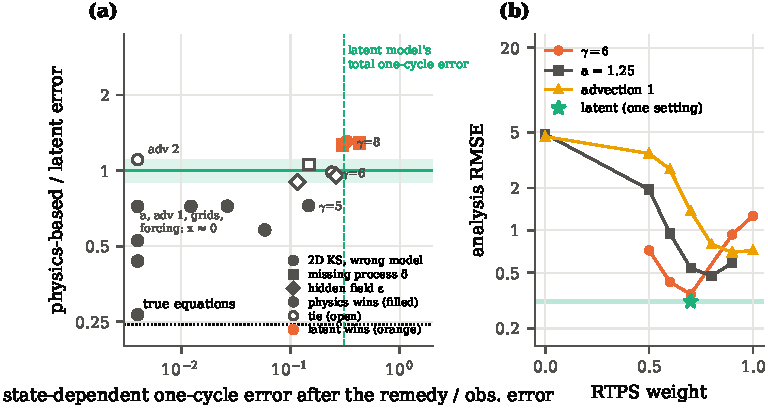
\includegraphics{figures/model_error.pdf}
\caption{Learned versus physics-based filters under model error, 2D KS at $44^2$. (a) The
physics-based filter's error over the latent filter's (three-seed means) against the state-dependent
part of its model's one-cycle forecast error (the part left after bias correction), in units of the
observation error; open: tuned RTPS and localization only; filled: with the best remedy (online
parameter estimation or bias correction); squares: the missing process ($\delta$), diamonds: the hidden
field ($\varepsilon$), each against its own latent model; the band marks $\pm10\%$ of the latent filter, the dotted line
a physics-based filter with the true equations. (b) The physics-based filter's error against its RTPS
weight for three wrong models (log scale; RTPS 0 diverged or was worse than interpolation), and the
latent filter's single setting. In this configuration, below a state-dependent one-cycle error of
about a sixth of the observation error the physics-based filter wins or ties; above it the latent
filter wins, except for the hidden field (diamonds), whose error the physics-based filter largely
removes by estimating the $\nabla^2$ coefficient; and the physics-based filter works only in a narrow
window of its tuning.}
\label{fig:model_error}
\end{figure*}


%======================================================================
\section{Trained only on noisy data}
%======================================================================
% TODO(S4.11): paper1 §7.6.
\placeholder{S4.11: Trained only on noisy data}

%======================================================================
\section{Forecasts, robustness, observation density and cost}
%======================================================================
% TODO(S4.12): paper1 §7.7, §7.9.
\placeholder{S4.12: Forecasts, robustness, observation density and cost}

%======================================================================
\section{The one-dimensional case}
%======================================================================
% TODO(S4.13): paper1 §7.8, Fig. 8.
\placeholder{S4.13: The one-dimensional case}

%======================================================================
\section{A second system: Kolmogorov flow}
%======================================================================
% TODO(SK6): new (Block SK).
\placeholder{SK6: A second system: Kolmogorov flow}

%======================================================================
\section{Discussion and limitations}
%======================================================================
% TODO(S4.14): paper1 §9 paras 5--6, limitation 6 expanded, new outlook.
\placeholder{S4.14: Discussion and limitations}

%======================================================================
\section{Conclusions}
\label{sec:conclusions}
%======================================================================

A learned latent field gives ensemble data assimilation in a latent space
what a latent vector cannot: a distance. With a decoder that reconstructs
each patch from its own site, the latent observation operator is exactly
local, so a per-site ensemble filter in the latent space is exact and its
observation Jacobian costs a fixed number of forward passes at any domain
size. The error that exact locality ties to the patch lattice is removed by
running the filter on four copies of the lattice shifted by half a patch
and blending them, which lowers the analysis error by about $30\%$ with the
same model.

Because the filter is local, neither its accuracy nor its ensemble depends
on the domain. With one model, trained only on noisy fields, and one
setting, it analyses two-dimensional Kuramoto--Sivashinsky fields to an
error of $0.30$--$0.33$ on every domain from $44^2$ to $440^2$, against $0.82$ for
interpolating the observations, with about 32 members per tiling, while an
unlocalized filter fails once the attractor has more unstable directions
than the ensemble has members. The same construction, with tilings shifted
only along the flow's symmetry, gives errors $43$--$44\%$ below interpolation in
Kolmogorov flow, on one box and on a domain three times wider.

Against a physics-based filter whose model is wrong, and which is given
online parameter estimation and bias correction, the latent filter loses
when the model's error is small or correctable and wins once the part of
that error which bias correction cannot remove exceeds about a sixth of the
observation error. That number, measured on chosen errors in one system,
is the quantity to estimate before replacing a physical model by a learned
one: where the structural error of the physical model is large and the
observations are good, a local model learned from noisy data is the better
forecast model for an ensemble filter, at any domain size.


\appendix
%======================================================================
\section{Model, training and filter settings}
%======================================================================
% TODO(S4.16): paper1 Table A last column, App. E.2--E.3.
\placeholder{S4.16: Model, training and filter settings}

%======================================================================
\section{Proof of Proposition 1}
%======================================================================
% TODO(S4.16): paper1 App. B.4.
\placeholder{S4.16: Proof of Proposition 1}

%======================================================================
\section{Ground truth}
\label{app:groundtruth}
%======================================================================

The protocol is that of Paper~I, which also validates the solvers; we
summarize what the 2D KS truths of Sec.~\ref{sec:ks2d} rest on.

\para{Lyapunov computation.} The base trajectory and $K$ tangent vectors
are advanced together by the same ETDRK4 step, the tangent vectors by the
exact Fr\'echet derivative of the right-hand side, which for
$\tfrac12|\nabla u|^2$ follows from the product rule without
approximation; the $\bm k=0$ mode is projected out of the base trajectory
and of every tangent vector. The tangent vectors are re-orthonormalized
by a QR factorization every time unit, and the exponents are the time
averages of $\log|R_{ii}|$ over a 40-unit window after a 20-unit warm-up,
which follows a spin-up of 200 time units. $K=150$ at $44^2$ and $300$ at $66^2$,
in both cases beyond the index at which the cumulative sum of exponents
turns negative, so $\DKY$ is computed, not extrapolated. The truths use
the grid of the model.

\para{Spread and convergence.} Three runs at $44^2$ give $81.8$, $80.7$ and
$83.6$, and two at $66^2$ give $192.5$ and $185.6$, a spread of $\pm1.8\%$ at both
sizes. Table~\ref{tab:running_ks2d} gives the running estimates of the runs
that recorded them: over the last 20 time units they still move by
$3$--$5\%$, in both directions. We therefore treat the truths as uncertain at
the level of a few percent, comparable to the model's errors in
Table~\ref{tab:model_validation}.

\begin{table}[htbp]
\caption{Running $\DKY$ of the 2D KS truth runs that recorded it, at the
averaging times shown (time units after the warm-up), and the change over
the last 20 time units.}
\label{tab:running_ks2d}
\begin{ruledtabular}
\begin{tabular}{lccccc}
run & 10 & 20 & 30 & 40 & last 20 \\
\hline
\tabinput{tables/running_ks2d}
\end{tabular}
\end{ruledtabular}
\end{table}

\para{Model spectra.} The model's spectrum is that of the latent map,
computed with the same algorithm: tangent vectors are propagated through
$\Fp$ by forward-mode automatic differentiation in single precision and
re-orthonormalized every 10 steps by a double-precision QR, with a warm-up
of 200 steps and $2000$ steps ($200$ time units), from the encoding of a true
state. We use $384$ tangent directions at $44^2$ and $512$ at $66^2$, again beyond
the index at which the cumulative sum turns negative. Paper~I shows that
double-precision propagation changes the 2D KS model's $\DKY$ by less than the
spread over initial conditions.

%======================================================================
\section{Data assimilation details}
%======================================================================
% TODO(S4.16): paper1 App. E.1, E.4--E.7.
\placeholder{S4.16: Data assimilation details}

%======================================================================
\section{Reproducibility}
%======================================================================
% TODO(S4.16): paper1 App. F, Part II code.
\placeholder{S4.16: Reproducibility}


\section*{Open Research Section}
% TODO(G5/S6.4): repository and DOI for code, trained models and the result files (user).
The code, the trained models, the result files that support the findings of this study and the
scripts that produce every table and figure from them (Appendix~\ref{app:reproducibility}) are
archived at \placeholder{repository and DOI, S6.4}.

\acknowledgments
% TODO(S6.3, user): funding, computing resources, and CRediT author contributions.
\placeholder{funding and author contributions}

\section*{Conflict of Interest}
The authors have no conflicts to disclose.

\bibliography{refs}

\end{document}
